% Options for packages loaded elsewhere
\PassOptionsToPackage{unicode}{hyperref}
\PassOptionsToPackage{hyphens}{url}
%
\documentclass[
]{article}
\usepackage{lmodern}
\usepackage{amssymb,amsmath}
\usepackage{ifxetex,ifluatex}
\ifnum 0\ifxetex 1\fi\ifluatex 1\fi=0 % if pdftex
  \usepackage[T1]{fontenc}
  \usepackage[utf8]{inputenc}
  \usepackage{textcomp} % provide euro and other symbols
\else % if luatex or xetex
  \usepackage{unicode-math}
  \defaultfontfeatures{Scale=MatchLowercase}
  \defaultfontfeatures[\rmfamily]{Ligatures=TeX,Scale=1}
\fi
% Use upquote if available, for straight quotes in verbatim environments
\IfFileExists{upquote.sty}{\usepackage{upquote}}{}
\IfFileExists{microtype.sty}{% use microtype if available
  \usepackage[]{microtype}
  \UseMicrotypeSet[protrusion]{basicmath} % disable protrusion for tt fonts
}{}
\makeatletter
\@ifundefined{KOMAClassName}{% if non-KOMA class
  \IfFileExists{parskip.sty}{%
    \usepackage{parskip}
  }{% else
    \setlength{\parindent}{0pt}
    \setlength{\parskip}{6pt plus 2pt minus 1pt}}
}{% if KOMA class
  \KOMAoptions{parskip=half}}
\makeatother
\usepackage{xcolor}
\IfFileExists{xurl.sty}{\usepackage{xurl}}{} % add URL line breaks if available
\IfFileExists{bookmark.sty}{\usepackage{bookmark}}{\usepackage{hyperref}}
\hypersetup{
  pdftitle={HarvardX PH125.9xData Science: Capstone: Movielens recommendation system},
  pdfauthor={Yannick Hermans},
  hidelinks,
  pdfcreator={LaTeX via pandoc}}
\urlstyle{same} % disable monospaced font for URLs
\usepackage[margin=1in]{geometry}
\usepackage{color}
\usepackage{fancyvrb}
\newcommand{\VerbBar}{|}
\newcommand{\VERB}{\Verb[commandchars=\\\{\}]}
\DefineVerbatimEnvironment{Highlighting}{Verbatim}{commandchars=\\\{\}}
% Add ',fontsize=\small' for more characters per line
\usepackage{framed}
\definecolor{shadecolor}{RGB}{248,248,248}
\newenvironment{Shaded}{\begin{snugshade}}{\end{snugshade}}
\newcommand{\AlertTok}[1]{\textcolor[rgb]{0.94,0.16,0.16}{#1}}
\newcommand{\AnnotationTok}[1]{\textcolor[rgb]{0.56,0.35,0.01}{\textbf{\textit{#1}}}}
\newcommand{\AttributeTok}[1]{\textcolor[rgb]{0.77,0.63,0.00}{#1}}
\newcommand{\BaseNTok}[1]{\textcolor[rgb]{0.00,0.00,0.81}{#1}}
\newcommand{\BuiltInTok}[1]{#1}
\newcommand{\CharTok}[1]{\textcolor[rgb]{0.31,0.60,0.02}{#1}}
\newcommand{\CommentTok}[1]{\textcolor[rgb]{0.56,0.35,0.01}{\textit{#1}}}
\newcommand{\CommentVarTok}[1]{\textcolor[rgb]{0.56,0.35,0.01}{\textbf{\textit{#1}}}}
\newcommand{\ConstantTok}[1]{\textcolor[rgb]{0.00,0.00,0.00}{#1}}
\newcommand{\ControlFlowTok}[1]{\textcolor[rgb]{0.13,0.29,0.53}{\textbf{#1}}}
\newcommand{\DataTypeTok}[1]{\textcolor[rgb]{0.13,0.29,0.53}{#1}}
\newcommand{\DecValTok}[1]{\textcolor[rgb]{0.00,0.00,0.81}{#1}}
\newcommand{\DocumentationTok}[1]{\textcolor[rgb]{0.56,0.35,0.01}{\textbf{\textit{#1}}}}
\newcommand{\ErrorTok}[1]{\textcolor[rgb]{0.64,0.00,0.00}{\textbf{#1}}}
\newcommand{\ExtensionTok}[1]{#1}
\newcommand{\FloatTok}[1]{\textcolor[rgb]{0.00,0.00,0.81}{#1}}
\newcommand{\FunctionTok}[1]{\textcolor[rgb]{0.00,0.00,0.00}{#1}}
\newcommand{\ImportTok}[1]{#1}
\newcommand{\InformationTok}[1]{\textcolor[rgb]{0.56,0.35,0.01}{\textbf{\textit{#1}}}}
\newcommand{\KeywordTok}[1]{\textcolor[rgb]{0.13,0.29,0.53}{\textbf{#1}}}
\newcommand{\NormalTok}[1]{#1}
\newcommand{\OperatorTok}[1]{\textcolor[rgb]{0.81,0.36,0.00}{\textbf{#1}}}
\newcommand{\OtherTok}[1]{\textcolor[rgb]{0.56,0.35,0.01}{#1}}
\newcommand{\PreprocessorTok}[1]{\textcolor[rgb]{0.56,0.35,0.01}{\textit{#1}}}
\newcommand{\RegionMarkerTok}[1]{#1}
\newcommand{\SpecialCharTok}[1]{\textcolor[rgb]{0.00,0.00,0.00}{#1}}
\newcommand{\SpecialStringTok}[1]{\textcolor[rgb]{0.31,0.60,0.02}{#1}}
\newcommand{\StringTok}[1]{\textcolor[rgb]{0.31,0.60,0.02}{#1}}
\newcommand{\VariableTok}[1]{\textcolor[rgb]{0.00,0.00,0.00}{#1}}
\newcommand{\VerbatimStringTok}[1]{\textcolor[rgb]{0.31,0.60,0.02}{#1}}
\newcommand{\WarningTok}[1]{\textcolor[rgb]{0.56,0.35,0.01}{\textbf{\textit{#1}}}}
\usepackage{graphicx,grffile}
\makeatletter
\def\maxwidth{\ifdim\Gin@nat@width>\linewidth\linewidth\else\Gin@nat@width\fi}
\def\maxheight{\ifdim\Gin@nat@height>\textheight\textheight\else\Gin@nat@height\fi}
\makeatother
% Scale images if necessary, so that they will not overflow the page
% margins by default, and it is still possible to overwrite the defaults
% using explicit options in \includegraphics[width, height, ...]{}
\setkeys{Gin}{width=\maxwidth,height=\maxheight,keepaspectratio}
% Set default figure placement to htbp
\makeatletter
\def\fps@figure{htbp}
\makeatother
\setlength{\emergencystretch}{3em} % prevent overfull lines
\providecommand{\tightlist}{%
  \setlength{\itemsep}{0pt}\setlength{\parskip}{0pt}}
\setcounter{secnumdepth}{-\maxdimen} % remove section numbering

\title{HarvardX PH125.9xData Science: Capstone: Movielens recommendation system}
\author{Yannick Hermans}
\date{1-10-2020}

\begin{document}
\maketitle

\hypertarget{introduction}{%
\subsection{Introduction}\label{introduction}}

In 2006 Netflix launched a competition where participants were asked to
optimize Netflix's movie recommendation system with at least 10 \%. The
winners were promised a prize worth \$1M. The challenge was to predict
user ratings as accurately as possible based on a dataset containing
previous user ratings. There was no additional knowledge on the users or
movies. In 2009 BellKor's Pragmatic Chaos team was able to best
Netflix's movie recommendation algorithm by 10.06\%

In this capstone project, which forms the conclusion to the HarvardX
PH125.9xData Science course, the goal is to build towards the
recommendation algorithm that the winners of the Netflix challenge
developed. This project will represent the knowledge I gained throughout
the EDX data science course on machine learning algorithms, data
processing and data exploration. A reduced version of the open source
MovieLens data set with 10M ratings, from 10,000 users on 72,000 movies,
has been used for this data science project.

This report contains the data processing steps, data exploratory
analysis and a few machine learning algorithms.

\hypertarget{data-preprocessing}{%
\subsection{Data preprocessing}\label{data-preprocessing}}

First the necessary packages are installed and loaded. The 10M MovieLens
dataset is loaded and separated into a training (``edx'') and a
validation ``validation'' set. The code for these preprocessing steps is
based on the already provided code in the edx capstone project module.
\url{https://courses.edx.org/courses/course-v1:HarvardX+PH125.9x+2T2018/courseware/dd9a048b16ca477a8f0aaf1d888f0734/e8800e37aa444297a3a2f35bf84ce452/?child=first}

\begin{Shaded}
\begin{Highlighting}[]
\CommentTok{#########################################################}
\CommentTok{# Create edx set, validation set (final hold_out test set)}
\CommentTok{#########################################################}

\CommentTok{# Note: this process could take a couple of minutes}

\ControlFlowTok{if}\NormalTok{(}\OperatorTok{!}\KeywordTok{require}\NormalTok{(tidyverse)) }\KeywordTok{install.packages}\NormalTok{(}\StringTok{"tidyverse"}\NormalTok{, }\DataTypeTok{repos =} \StringTok{"http://cran.us.r-project.org"}\NormalTok{)}
\ControlFlowTok{if}\NormalTok{(}\OperatorTok{!}\KeywordTok{require}\NormalTok{(caret)) }\KeywordTok{install.packages}\NormalTok{(}\StringTok{"caret"}\NormalTok{, }\DataTypeTok{repos =} \StringTok{"http://cran.us.r-project.org"}\NormalTok{)}
\ControlFlowTok{if}\NormalTok{(}\OperatorTok{!}\KeywordTok{require}\NormalTok{(data.table)) }\KeywordTok{install.packages}\NormalTok{(}\StringTok{"data.table"}\NormalTok{, }\DataTypeTok{repos =} \StringTok{"http://cran.us.r-project.org"}\NormalTok{)}

\KeywordTok{library}\NormalTok{(tidyverse)}
\KeywordTok{library}\NormalTok{(caret)}
\KeywordTok{library}\NormalTok{(data.table)}

\CommentTok{# MovieLens 10M dataset:}
\CommentTok{# https://grouplens.org/datasets/movielens/10m/}
\CommentTok{# http://files.grouplens.org/datasets/movielens/ml-10m.zip}

\NormalTok{dl <-}\StringTok{ }\KeywordTok{tempfile}\NormalTok{()}
\KeywordTok{download.file}\NormalTok{(}\StringTok{"http://files.grouplens.org/datasets/movielens/ml-10m.zip"}\NormalTok{, dl)}
\NormalTok{ratings <-}\StringTok{ }\KeywordTok{fread}\NormalTok{(}\DataTypeTok{text =} \KeywordTok{gsub}\NormalTok{(}\StringTok{"::"}\NormalTok{, }\StringTok{"}\CharTok{\textbackslash{}t}\StringTok{"}\NormalTok{, }\KeywordTok{readLines}\NormalTok{(}\KeywordTok{unzip}\NormalTok{(dl, }\StringTok{"ml-10M100K/ratings.dat"}\NormalTok{))),}
                 \DataTypeTok{col.names =} \KeywordTok{c}\NormalTok{(}\StringTok{"userId"}\NormalTok{, }\StringTok{"movieId"}\NormalTok{, }\StringTok{"rating"}\NormalTok{, }\StringTok{"timestamp"}\NormalTok{))}

\NormalTok{movies <-}\StringTok{ }\KeywordTok{str_split_fixed}\NormalTok{(}\KeywordTok{readLines}\NormalTok{(}\KeywordTok{unzip}\NormalTok{(dl, }\StringTok{"ml-10M100K/movies.dat"}\NormalTok{)), }\StringTok{"}\CharTok{\textbackslash{}\textbackslash{}}\StringTok{::"}\NormalTok{, }\DecValTok{3}\NormalTok{)}
\KeywordTok{colnames}\NormalTok{(movies) <-}\StringTok{ }\KeywordTok{c}\NormalTok{(}\StringTok{"movieId"}\NormalTok{, }\StringTok{"title"}\NormalTok{, }\StringTok{"genres"}\NormalTok{)}

\NormalTok{movies <-}\StringTok{ }\KeywordTok{as.data.frame}\NormalTok{(movies) }\OperatorTok\StringTok{ }\KeywordTok{mutate}\NormalTok{(}\DataTypeTok{movieId =} \KeywordTok{as.numeric}\NormalTok{(movieId),}
                                           \DataTypeTok{title =} \KeywordTok{as.character}\NormalTok{(title),}
                                           \DataTypeTok{genres =} \KeywordTok{as.character}\NormalTok{(genres))}

\NormalTok{movielens <-}\StringTok{ }\KeywordTok{left_join}\NormalTok{(ratings, movies, }\DataTypeTok{by =} \StringTok{"movieId"}\NormalTok{)}

\CommentTok{# Validation set will contain 10% of the MovieLens data set}
\KeywordTok{set.seed}\NormalTok{(}\DecValTok{1}\NormalTok{, }\DataTypeTok{sample.kind =} \StringTok{"Rounding"}\NormalTok{)}
\NormalTok{test_index <-}\StringTok{ }\KeywordTok{createDataPartition}\NormalTok{(}\DataTypeTok{y =}\NormalTok{ movielens}\OperatorTok{$}\NormalTok{rating, }\DataTypeTok{times =} \DecValTok{1}\NormalTok{, }\DataTypeTok{p =} \FloatTok{0.1}\NormalTok{, }\DataTypeTok{list =} \OtherTok{FALSE}\NormalTok{)}
\NormalTok{edx <-}\StringTok{ }\NormalTok{movielens[}\OperatorTok{-}\NormalTok{test_index,]}
\NormalTok{temp <-}\StringTok{ }\NormalTok{movielens[test_index,]}
\CommentTok{# Make sure userId and movieId in validation set are also in edx set}
\NormalTok{validation <-}\StringTok{ }\NormalTok{temp }\OperatorTok
\StringTok{  }\KeywordTok{semi_join}\NormalTok{(edx, }\DataTypeTok{by =} \StringTok{"movieId"}\NormalTok{) }\OperatorTok
\StringTok{  }\KeywordTok{semi_join}\NormalTok{(edx, }\DataTypeTok{by =} \StringTok{"userId"}\NormalTok{)}
\CommentTok{# Add rows removed from validation set back into edx set}
\NormalTok{removed <-}\StringTok{ }\KeywordTok{anti_join}\NormalTok{(temp, validation)}
\NormalTok{edx <-}\StringTok{ }\KeywordTok{rbind}\NormalTok{(edx, removed)}

\KeywordTok{rm}\NormalTok{(dl, ratings, movies, test_index, temp, movielens, removed)}
\end{Highlighting}
\end{Shaded}

The validation set is used to determine the accuracy of the final movie
recommendation algorithm. The other models are tested by splitting up
the edx set into a training (edx\_training\_set) and a test set
(edx\_test\_set).

\begin{Shaded}
\begin{Highlighting}[]
\CommentTok{# Split edx data in training (80%) and test set (20%) }
\KeywordTok{set.seed}\NormalTok{(}\DecValTok{1992}\NormalTok{, }\DataTypeTok{sample.kind =} \StringTok{"Rounding"}\NormalTok{)}
\NormalTok{edx_test_index <-}\StringTok{ }\KeywordTok{createDataPartition}\NormalTok{(}\DataTypeTok{y =}\NormalTok{ edx}\OperatorTok{$}\NormalTok{rating, }\DataTypeTok{times =} \DecValTok{1}\NormalTok{,}
                                  \DataTypeTok{p =} \FloatTok{0.2}\NormalTok{, }\DataTypeTok{list =} \OtherTok{FALSE}\NormalTok{)}
\NormalTok{edx_train_set <-}\StringTok{ }\NormalTok{edx[}\OperatorTok{-}\NormalTok{edx_test_index,]}
\NormalTok{edx_test_set <-}\StringTok{ }\NormalTok{edx[edx_test_index,]}

\NormalTok{edx_test_set <-}\StringTok{ }\NormalTok{edx_test_set }\OperatorTok
\StringTok{  }\KeywordTok{semi_join}\NormalTok{(edx_train_set, }\DataTypeTok{by =} \StringTok{"movieId"}\NormalTok{) }\OperatorTok
\StringTok{  }\KeywordTok{semi_join}\NormalTok{(edx_train_set, }\DataTypeTok{by =} \StringTok{"userId"}\NormalTok{)}
\end{Highlighting}
\end{Shaded}

In addition, certain libraries for the data exploration and machine
learning development are loaded

\begin{Shaded}
\begin{Highlighting}[]
\KeywordTok{library}\NormalTok{(lubridate)}
\KeywordTok{library}\NormalTok{(ggplot2)}
\KeywordTok{library}\NormalTok{(recosystem)}
\end{Highlighting}
\end{Shaded}

\hypertarget{data-exploratory-analysis}{%
\subsection{Data exploratory analysis}\label{data-exploratory-analysis}}

First an onverview of the data is given

\begin{Shaded}
\begin{Highlighting}[]
\KeywordTok{head}\NormalTok{(edx)}
\end{Highlighting}
\end{Shaded}

\hypertarget{recommendation-algorithm-development}{%
\subsection{Recommendation algorithm
development}\label{recommendation-algorithm-development}}

\hypertarget{strategy}{%
\subsubsection{Strategy}\label{strategy}}

\hypertarget{model-1}{%
\subsubsection{Model 1:}\label{model-1}}

\hypertarget{model-2}{%
\subsubsection{Model 2:}\label{model-2}}

\hypertarget{model-3}{%
\subsubsection{Model 3:}\label{model-3}}

\hypertarget{model-4}{%
\subsubsection{Model 4:}\label{model-4}}

\hypertarget{model-5}{%
\subsubsection{Model 5:}\label{model-5}}

\hypertarget{model-6}{%
\subsubsection{Model 6:}\label{model-6}}

\hypertarget{model-7}{%
\subsubsection{Model 7:}\label{model-7}}

\hypertarget{r-markdown}{%
\subsection{R Markdown}\label{r-markdown}}

This is an R Markdown document. Markdown is a simple formatting syntax
for authoring HTML, PDF, and MS Word documents. For more details on
using R Markdown see \url{http://rmarkdown.rstudio.com}.

When you click the \textbf{Knit} button a document will be generated
that includes both content as well as the output of any embedded R code
chunks within the document. You can embed an R code chunk like this:

\begin{Shaded}
\begin{Highlighting}[]
\KeywordTok{summary}\NormalTok{(cars)}
\end{Highlighting}
\end{Shaded}

\begin{verbatim}
##      speed           dist       
##  Min.   : 4.0   Min.   :  2.00  
##  1st Qu.:12.0   1st Qu.: 26.00  
##  Median :15.0   Median : 36.00  
##  Mean   :15.4   Mean   : 42.98  
##  3rd Qu.:19.0   3rd Qu.: 56.00  
##  Max.   :25.0   Max.   :120.00
\end{verbatim}

\hypertarget{including-plots}{%
\subsection{Including Plots}\label{including-plots}}

You can also embed plots, for example:

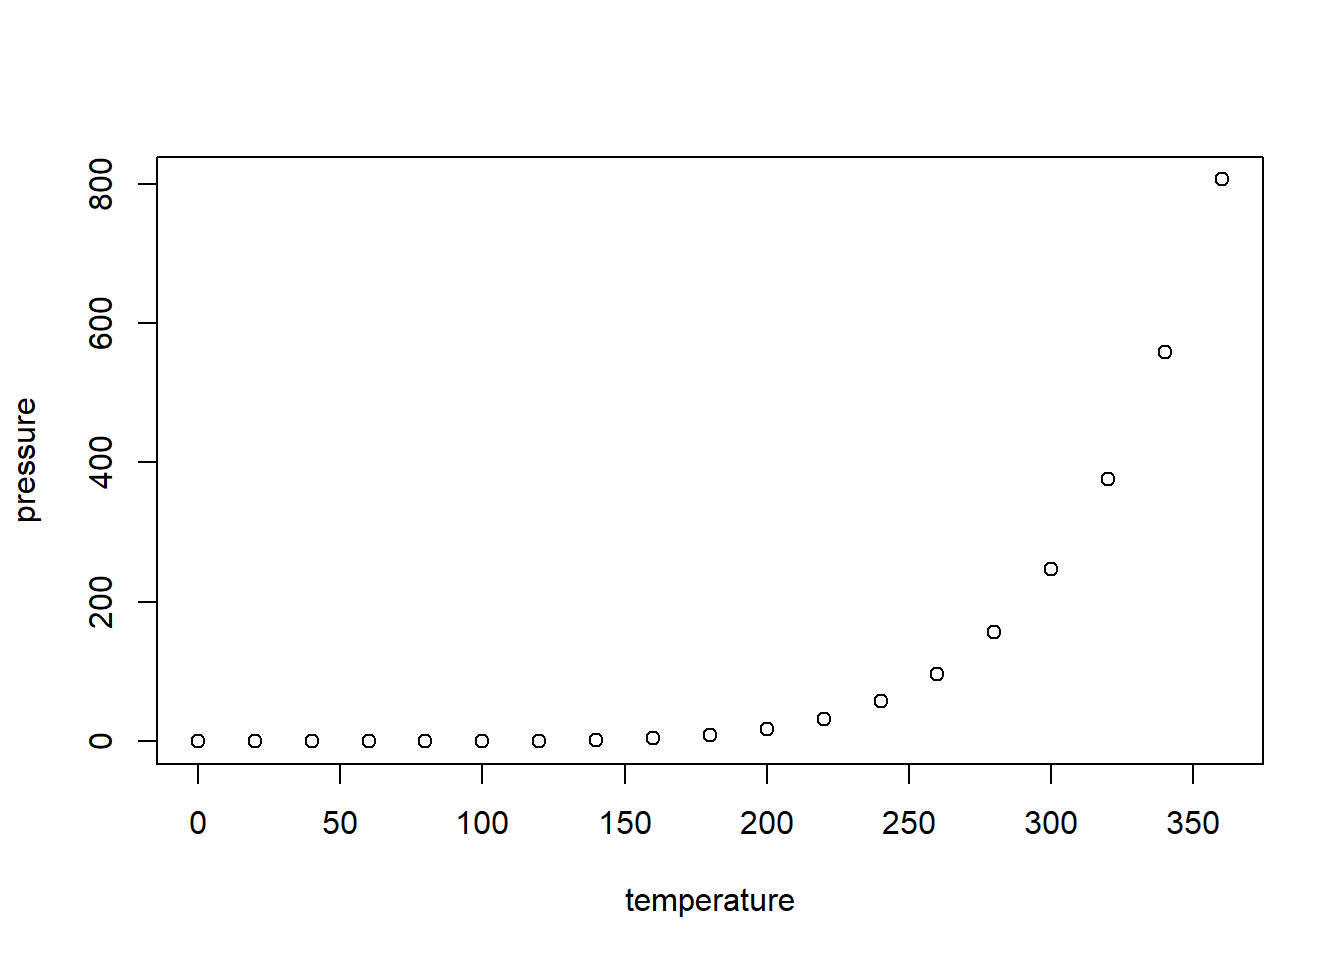
\includegraphics{Movielens_project_files/figure-latex/pressure-1.pdf}

Note that the \texttt{echo\ =\ FALSE} parameter was added to the code
chunk to prevent printing of the R code that generated the plot.

\end{document}
